%%%%%%%%%%%%%%%%%%%%%%%%%%%%%%%%%%%%%%%%%%%%%%%%%%%%%%%%%%%%%%%%%%%%%%%%%%%%%%%%
%2345678901234567890123456789012345678901234567890123456789012345678901234567890
%        1         2         3         4         5         6         7         8

\documentclass[letterpaper, 10 pt, conference]{ieeeconf}  % Comment this line out
\IEEEoverridecommandlockouts


\usepackage[ngerman]{babel}
\usepackage{paralist, tabularx}
\usepackage{subfigure}
\usepackage{amsmath}

\usepackage{soul}
\usepackage{xcolor}
\newcommand\sichen[1]{\textcolor{red}{sichen: #1}}
\newcommand\siqi[1]{\textcolor{blue}{siqi: #1}}
\title{\LARGE \bf
Data Plane Verification as Program Verification
}


\author{Siqi Liu,
Sichen Song
}

\usepackage[T1]{fontenc}
\usepackage{graphicx}
\usepackage{listings}
\begin{document}



\maketitle
\thispagestyle{empty}
\pagestyle{empty}



\section{INTRODUCTION}
Data plane verification is an emerging field of computer networking, in which the behavior of network data plane is verified to follow a specification. 

To perform data plane verification, the network topology and forwarder configurations are typically encoded into a model, which is checked against the specification. For example, the Header Space Analysis (HSA) encodes the network nodes into functions on packet state, which consists of packet header and packet location~\cite{hsa}. HSA then simulates a symbolic packet being forwarded through the network model to verify reachability and other properties. Anteater, on the other hand, models the network and its specification as SAT formulas on the packet header and reduces the network verification problem into a SAT problem, which can be solved using existing SAT solvers such as Z3~\cite{z3}.

The existing works focuses on verifying stateless network nodes and consequently does not work on networks with stateful load balancers or NAT boxes. Although data plane specification language has been proposed in NoD~\cite{nod} and NetPlumber~\cite{netp}, the languages has limited expressiveness and requires times for network operators to learn. Lastly, the generated model is hard to understand or debug due to extensive use of logical formulas.

To address the above issues, we investigation into modeling the data plane as a computer program and utilizing existing symbolic execution tool, KLEE~\cite{klee}, to verify network properties. In the following sections, we provide the feasibility of reducing network verification into a program verification in \S~\ref{sec:feasibility}. We then present the architecture of our verifier that reduce network verification into program verification in \S ~\ref{sec:overall}. We dive into details of code generation in \S~\ref{sec:codegen}. We also propose potential optimizations that could potentially use pre-computation to improve the performance of verification in \S~\ref{sec:opt}. Lastly we discuss the evaluation results in \S~\ref{sec:eval}.


\section{Feasibility Analysis}\label{sec:feasibility}

Symbolic execution for program verification models program input as a set of potential values and explores the control flow graph of the program by executing the program and adding path constrains to the symbolic variables whenever having conditional statements. By keeping track of a set of potential input that leads to certain execution path, feasibility of  execution path can be calculated by checking whether the path conditions is satisfiable. In this way, by exploring all reachable execution paths, the program can be verified.

Symbolic execution is similar to Header Space Analysis(HSA) as they both use equivalence classes of input to ensure efficient and comprehensive exploration a directed graph. Both of them also reason about reachability in the graph by transforming the problem as a satisfiability problem of path condition.

This similarity motivates us to explore the idea of transforming the network verification problem into a program verification problem and transform network reachability and other properties to verify into code reachability. The idea can be implemented by generating the network configuration and verification problem into a network simulator on symbolic packet inputs. This reduction can have the following advantages:

\begin{enumerate}
  \item The generated model is a network simulator written in C++, which is easier to understand and debug compared to logical formula based modeling.
  \item Existing optimizer in compiler such as constant propagation and dead code elimination can operate on the generated code.
  \item Stateful nodes such as NAT can be modeled as a mutable objects that forward packets.
  \item The specification is essentially C++ code operating on packet state or path, which is easier to learn by network operators.
  \item The generated network simulator can be executed with concrete packet input, which can be reused to debug network configurations by visualizing packet forwarding.
\end{enumerate}

However, verifying data plane relying on program verification has the following disadvantages:

\begin{enumerate}
 \item Existing program verification tools are used as black boxes. Consequently there's less opportunity to apply domain knowledge to fine tune the implementation details for optimization.
 \item Program verification solves path constrains with SMT solver such as Z3, which only gives a single example for each property violation.
\end{enumerate}

\section{Overall Design}\label{sec:overall}
The overall design of our network verification framework is illustrated in fig.~\ref{fig:arch}. 

To reduce data plane verification into program verification, code generation is extensively used. Overall there are three different types of code generators: the network node generator, the topology generator, and verification generator. Network node generator generates forwarders and other nodes in the network from its configurations such as FIBs and ACLs. A variety of node types is supported such as ECMP routers and stateful NAT boxes. Topology generator generates the code that takes a packet state (header, location) as input and move a packet through the network for one step. The packet is first fed into the corresponding forwarder to make a forwarding action. The output packet is then transformed into a input packet of the next hop by looking up the network topology. Lastly, the verification generator will generate the "main function" that injects symbolic packets into the network and keep forwarding it through the network. The most import part of it is the main loop that keeps forwarding packets step by step using the topology generator. Depending on the property to verify, the generator may also record of packet paths and other states for later property checks. The code generators may embed comments in the generated code to facilitate post-processing.

These generated C++ code will be compiled into LLVM intermediate representation (IR) using the LLVM C++ front end Clang++. These IR is then used by KLEE for symbolic execution. KLEE will invoke LLVM optimization passes on the input IR and symbolically execute the program to maximize line coverage and check if it can fail any assertion in the program. The resulting coverage file is then fed into a post processing script to check if the property-to-verify is maintained by the network. The generated comments by code generators acts has hints for the post processor to better understand the coverage and thus make verification decisions.

\begin{figure}[]
  \centering
  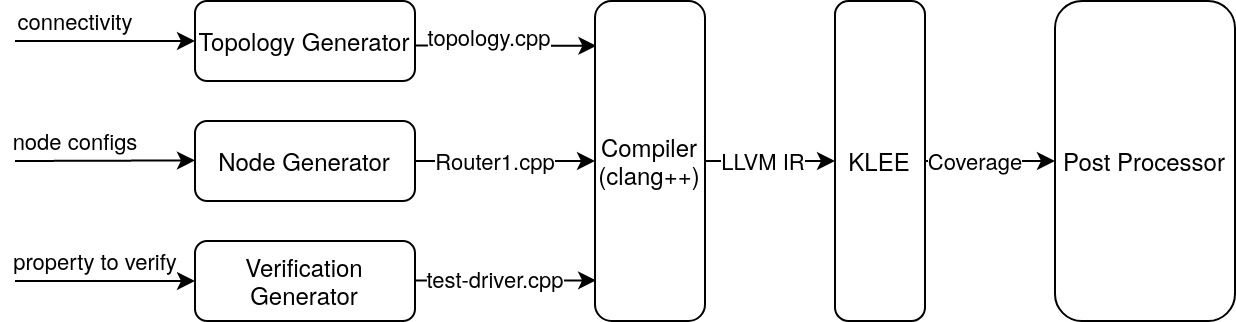
\includegraphics[width=\linewidth]{overview.png}
  \caption{Architecture}
  \label{fig:arch}
\end{figure}

\section{Code Generation}\label{sec:codegen}
Code generator is the primary part of reducing data plane verification into program verification. The generators will generate a  executable C++ program that asserts the property-to-verify with symbolic packet inputs such that symbolic execution can later be used to check these assertions. The code is also annotated with generated comments serving as hints to help the poster processor to translate code coverage report from KLEE into network verification results.
\subsection{Constrains}
Symbolic execution can perform poorly when the program has large loops, requires variable length in-memory data structures, or make many unnecessary branches. Being aware of these limitations, code generator of this framework inlines table (for example, FIB) lookup as a sequence of branches, instead of relying on in-memory data structures. It also bounds all loops to bound the total amount of execution paths. 

\subsection{Packet State}
Inspired by HSA~\cite{hsa}, the packet state is the combination of header and location as shown in listing \ref{code:state}.
\begin{lstlisting}[language=C,caption=Packet State,label=code:state,captionpos=b]
struct Header {
  uint32_t src_address;
  uint32_t dst_address;
...
};

struct PktState {
  Header header;
  int node;
  int port;
};
\end{lstlisting}

\subsection{Stateless Network Routers}
Stateless network Routers are generated based on their FIB and ACL configurations. An C++ class with the node name is generated that has a \emph{forward} method that transforms the input packet state to the output packet state. Listing~\ref{code:stateless-router} shows a generated router class. Note that a linear scan over the routing table from longest prefix to shortest prefix is used for FIB lookup, which may result in poor performance. Optimization of FIB lookup is discussed in sec.~\ref{sec:opt}. Also, the \emph{[reached] Router4} comment act as a hint to facilitate post processing of node reachability.

\begin{lstlisting}[
  language=C,
  caption=generated stateless router,
  label=code:stateless-router,
  captionpos=b,
  basicstyle=\small]
class Router4 {
  public:
  
  PktState 
  forward(PktState stateIn) { //[reached] Router4
    int node = stateIn.node;
    int portIn = stateIn.port;
    Header &header = stateIn.header;
    int portOut = forwardTable(header.dst_address);
    if (!acl(header, portIn, portOut)) 
        return {header, node, -1};
    return {header, node, portOut};
  }
  
  int forwardTable(uint32_t dst) {
  if ((dst >> 16) == (0xa000000 >> 16))//10.0.0.0/16
    return 1;
  if ((dst >> 16) == (0xa010000 >> 16))//10.1.0.0/16
    return 2;
  return -1;
    ...
  }
  
  bool acl(Header header, int ingress, int egress) {
    if (
    header.dst_port == 80 &&
    header.protocol == 6 &&
    true)
      return false; // DenyHTTP
    ...
    return true; // false as drop
  }
};
\end{lstlisting}


\subsection{Network}

The network with connectivity and node is generated as a C++ class, which instantiates all the nodes and expose a function that takes a packet state and makes one step of packet forwarding. The input packet is first processed by the corresponding forwarder to be transformed to an output packet. Then, by looking up network connectivity, the output packet is moved to the input port of the other end of the link.  Listing~\ref{code:topology} shows a generated network class.

\begin{lstlisting}[  language=C,
  caption=generated network class,
  label=code:topology,
  captionpos=b,
  basicstyle=\small]
class Topology {
  public:
  
  PktState 
  node_execute(PktState pktState) {
    int node = pktState.node;
    Header &header = pktState.header;
    int port = pktState.port;
    if (node == 0) {
      return node0.forward(pktState);
    }
    ...
    
    assert(0); //[node-dispatch-failed]
  }
  
  static PktState 
  link_function(PktState in) {
    int node = in.node;
    int port = in.port;
    Header &header = in.header;
    if (node == 0 && port == 1)
    return {header, 1, 1};
    if (node == 1 && port == 1)
    return {header, 0, 1};
    ...
  }
  
  public:
  Router1 node0;
  Router2 node1;
...
};
\end{lstlisting}

\subsection{Reachability Query Test Driver}
The reachability query test driver simply injects a symbolic packet at the user-selected node and simulate the packet forwarding until the packet exits or TTL runs out. KLEE will enumerate the entire header space trying to cover every line of code, which includes the forward method of each node object. Thus, the coverage report of KLEE can be used to infer if a node is reachable by checking if its corresponding class and method is covered. To cover a reasonable number of packet forwarding while bounding the main loop for packet forwarding, we set the TTL to be two times the diameter of the network topology.
Listing~\ref{code:reachability-driver} shows a generated reachability test driver. It can be seen that this test driver prints out the path a packet traverses when a concrete packet is used to run simulation. 

\begin{lstlisting}[  language=C,
  caption=generated reachability/loop test driver,
  label=code:reachability-driver,
  captionpos=b,
  basicstyle=\small]
class Network : public Topology {
  public:
  void forward(PktState pktState) {
    if (klee_is_replay())
      printf("Starting port: %d %d\n"...);
    for (int hop = 0; hop < 6; hop++) {
      PktState forwardedPktState = 
        node_execute(pktState);
      if (forwardedPktState.port == PORT_DROP) {
        if (klee_is_replay())
          printf("Drop by: %d %d\n"...);
        return;
      }
      pktState = link_function(forwardedPktState);
      if (klee_is_replay())
        printf("Forward to: %d %d => %d %d\n"...);
      if (pktState.port == PORT_DROP) return;
    }
    assert(0); //[TTL-Drop] potential loop
    return;
  }
};

int main() {
  Header header;
  klee_make_symbolic(&header, 
   sizeof(header), "header");
  
  Network n;
  n.forward(PktState(header,Router1Id,0));
  
  return 0;
}
\end{lstlisting}

\subsection{Loop Detection Query}
Intuitively, loop detection should check if a packet reenters a router. However, to minimize the states and simplify the problem, we detect loop by checking for TTL violations. By settings a TTL much larger than network diameter and checking for TTL drop. Loops can be detected. The loop detection test driver is exactly the same as the reachability query test driver in listing~\ref{code:reachability-driver}. Note that the generated comment \emph{[TTL-Drop] potential loop} is used for post processors to identify the test packet that could trigger loop.
\subsection{Stateful Nodes}
\siqi{todo}
\subsection{Other Queries}
\siqi{todo or remove section}
\subsection{Optimization}\label{sec:opt}
The goal of optimization in code generation is to reduce unnecessary number of instructions, especially branches. Our optimization focuses on the common case of longest prefix matching based stateless routers without ACL or ECMP. There are two aspects of optimization we hope to achieve. Firstly, the routing table lookup has lots of branches and we hope to improve the performance by both compressing and aggregating the routing table while using a efficient lookup algorithm. Secondly, a group of routers can be replaced as a single node with the same behavior from the outside point of view. This grouping of nodes and abstracting them as a single one allows joint optimization and lookup of all the routing tables in this group.

To achieve this goal, equivalence classes are first generated from routing tables of the selected group of nodes using atomic predicate~\cite{ap}. Then, a concrete packet of each equivalence class is injected to each the nodes in the group in the generated network simulator to find where packets of the equivalence class exits the group. Lastly, giving a set of <equivalence class, input node, output node, output port>, we generate a C++ Router class that forwards the packet by looking up a equivalence class based lookup table using binary search on ranges~\cite{binary_search_lookup}.

Figure~\ref{fig:opt} shows the implementation of the optimization procedure. Other than the network configuration, the user also specify a group of nodes to act as a ``module'' or ``component'' that will be optimized to a single node. Equivalence classes will be generated first using a bit trie with the idea of aptomic predicate. For each of the equivalence class, a concrete packet is also generated. With these information, a network simulator will be generated that injects a concrete packet of each equivalence class to each node in the group. The execution of the simulator will record where each of these injected packet exits the group of nodes. This output is then used to generate a single node class that make forwarding decision by looking up the input equivalence class using binary search on ranges.

By merging consecutive ranges having the same forwarding result before generating code for binary search, the routing table can effectively be compressed and aggregated.

\begin{figure}[]
 \centering
 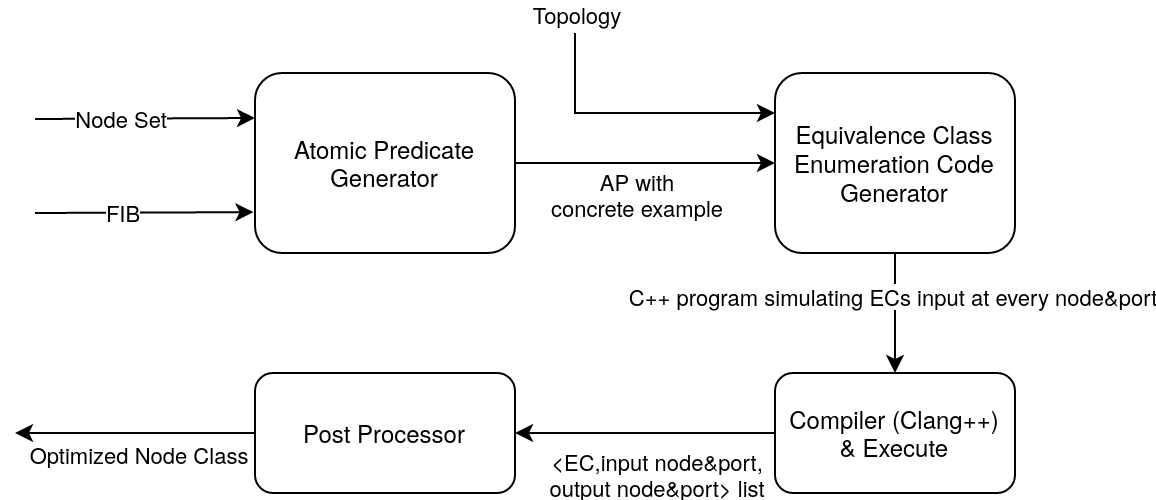
\includegraphics[width=\linewidth]{optimization.png}
 \caption{Optimization Implementation}
 \label{fig:opt}
\end{figure}

Listing~\ref{code:opt} shows a generated optimized router class. The nested if are the inlined binary search procedure.

\begin{lstlisting}[  language=C,
 caption=Optimization of Router: Binary Search on Ranges,
 label=code:opt,
 captionpos=b,
 basicstyle=\tiny]
class LeafP19S3 {
 public:
 PktState forward(PktState stateIn) { //generated-comment: [reached] LeafP19S3
  int node = stateIn.node;
  int portIn = stateIn.port;
  Header &header = stateIn.header;
  if (header.dst_address >= 0xa130600 && header.dst_address <= 0xa1306ff)
  return {header, 449, -1};
  else if (header.dst_address < 0xa130600) {
   if (header.dst_address >= 0xa130200 && header.dst_address <= 0xa1302ff)
   return {header, 445, -1};
   else if (header.dst_address < 0xa130200) {
    if (header.dst_address >= 0xa130000 && header.dst_address <= 0xa1300ff)
    return {header, 435, -1};
    else if (header.dst_address < 0xa130000) {
     return {header, 435, 12};
    } else {
     return {header, 432, -1};
    }
   } else {
    if (header.dst_address >= 0xa130400 && header.dst_address <= 0xa1304ff)
    return {header, 447, -1};
    else if (header.dst_address < 0xa130400) {
     return {header, 446, -1};
    } else {
     return {header, 448, -1};
    }
   }
  } else {
   if (header.dst_address >= 0xa130a00 && header.dst_address <= 0xa130aff)
   return {header, 453, -1};
   else if (header.dst_address < 0xa130a00) {
    if (header.dst_address >= 0xa130800 && header.dst_address <= 0xa1308ff)
    return {header, 451, -1};
    else if (header.dst_address < 0xa130800) {
     return {header, 450, -1};
    } else {
     return {header, 452, -1};
    }
   } else {
    if (header.dst_address >= 0xa130c00 && header.dst_address <= 0xa130cff)
    return {header, 455, -1};
    else if (header.dst_address < 0xa130c00) {
     return {header, 454, -1};
    } else {
     if (header.dst_address >= 0xa140000)
     return {header, 435, 12};
     return {header, 435, -1};
     
    }
   }
  }
  assert(0);
 }
};

\end{lstlisting}
\section{Evaluation}\label{sec:eval}
The data plane verification design is evaluated for both its performance and correctness.

\begin{figure}[]
	\centering
	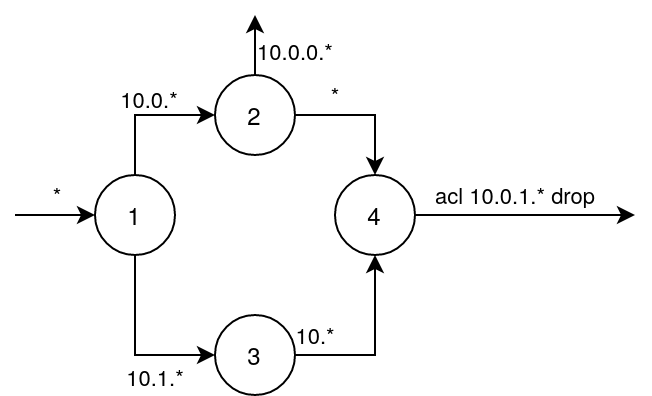
\includegraphics[width=\linewidth]{scenario-simple.png}
	\caption{4-node topology}
	\label{fig:scenario1}
\end{figure}

\subsection{stateful nodes}

\subsection{optimization}
The optimization is evaluated in two scenarios. First, the effectiveness of FIB compression is evaluated in a 4-node topology illustrated by Fig.~\ref{fig:scenario1}. To show the effectiveness of routing table compression, we divided the two length 16 prefixes in forwarding table of node 1 to 2048 length 26 prefixes. We then run a source reachability query from node 1 with or without optimization and record the execution time of compilation and KLEE symbolic execution. Secondly, the efficiency of joint optimization across multiple nodes by grouping them into a single node is evaluated in a fat tree topology with 720 routers. The optimizer groups each pod of the fat tree into a single node. A source reachability query is run from one leaf node toward all other nodes. Table~\ref{tab:eval-opt} shows the result of the evaluations. The path row shows number of execution paths KLEE discovered and the instructions row shows the number of instructions executed during the symbolic execution.

The result for the routing table compression is promising. The execution time is improved for more than 100 times. Looking at the number of path and instructions explored by symbolic execution, we can see that by merging routing table entries, the number of paths in the program is significantly reduced, which contributes to the performance gain.

The result for the grouping, however, shows that the optimization is \textbf{not} useful. While the number of instruction executed by KLEE is significantly reduced, the number of paths and running time is not. That's because in the fat tree, there's no redundant routing rules and thus the optimization does not improve much on the number of path symbolic execution must explore. This also suggests that pruning the path has much higher performance gain compared with reducing the number of instructions.
\begin{table}[!ht]
	\centering
	\begin{tabular}{|l|l|l|l|l|}
		\hline
		scenario & 4-node & 4-node & fat-tree & fat-tree  \\ \hline
		optimization & no & yes & no & yes  \\ \hline
		time & 85.62s & 0.22s & 76.57s & 71.92s \\ \hline
		path & 1119 & 7 & 313 & 338 \\ \hline
		instructions & 1106328 & 3205 & 2606934 & 367028 \\ \hline
	\end{tabular}
	\caption{optimization evaluation results}
	\label{tab:eval-opt}
\end{table}

\section{FUTURE DIRECTION}\label{sec:fd}

\section{CONCLUSIONS}\label{sec:c}




\addtolength{\textheight}{-12cm}  
\bibliographystyle{IEEEtran}
\bibliography{bibs}


\end{document}

